\begin{figure}[htbp]
\centering
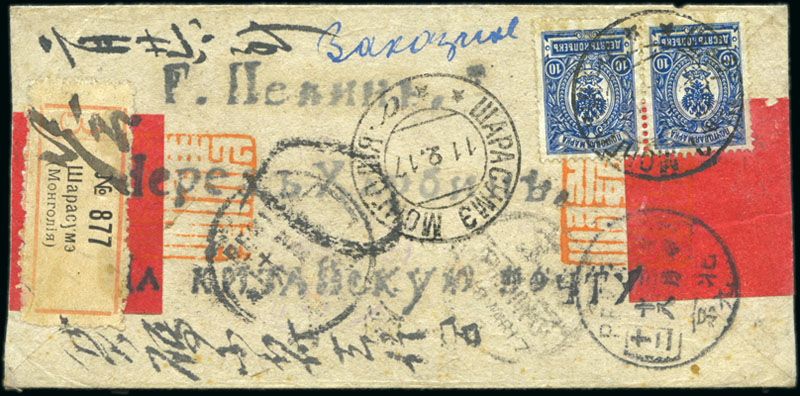
\includegraphics[width=.95\textwidth]{../russian-post-in-mongolia/10150.jpg}
\caption{ 
10150 SHARASUME: 1917 Native cover sent registered to Peking, franked with 10k
blue pair paying the 10k single rate plus registration, tied by Sharasume 11.2.17 cds,
with registration label adjacent (type not recorded by Hellrigl), 
fine and rare registered cover.
\euro 1,800.00 
} 
\end{figure}  

\begin{figure}[htbp]
\centering
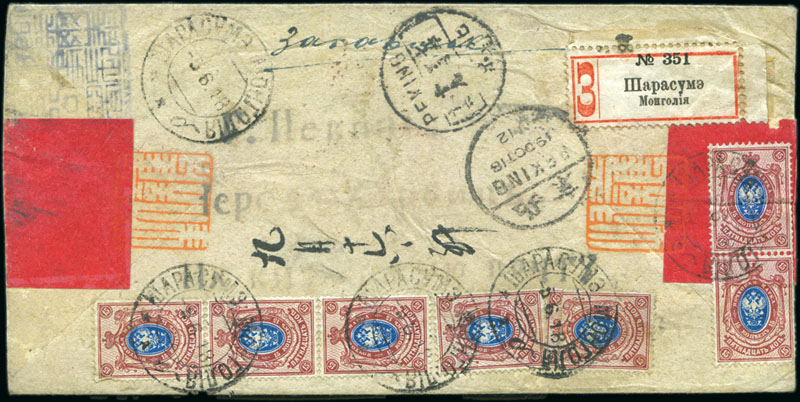
\includegraphics[width=.95\textwidth]{../russian-post-in-mongolia/10151.jpg}
\caption{ 
10151 SHARASUME: 1918 Native cover sent registered to Peking, with seven 15k blue 
\& plum tied by Sharasume 5.6.18 cds, with registration label adjacent 
(Hellrigl type 1 rated R, later use than recorded), fine and 
rare multiple franking.
Provenance: Ex Adgey-Edgar
Currently (SAN) \euro1,800.00 
} 
\end{figure}

\begin{figure}[htbp]
\centering
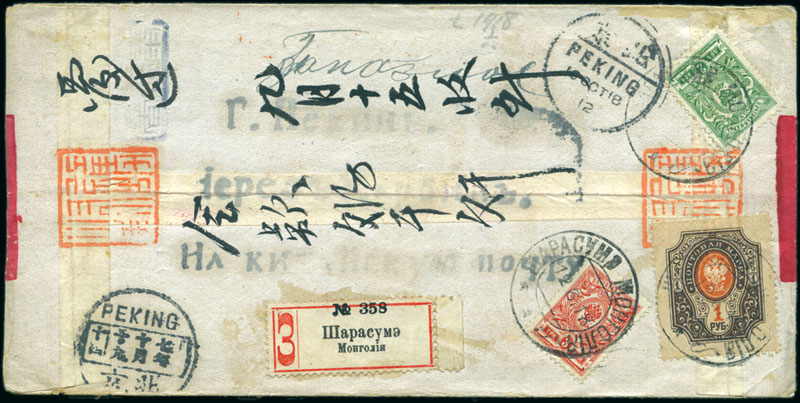
\includegraphics[width=.95\textwidth]{../russian-post-in-mongolia/10152.jpg}
\caption{ 
10152	SHARASUME: 1918 Native cover sent registered to Peking, with 2k, 3k and 
1R tied by Sharasume 12.6.18 cds, with registration label adjacent 
(Hellrigl type 1 rated R, later use than recorded), with Russian and Chinese
Peking arrival ds after more than four months in transit, a rare high franking.
\euro 1,800.00
} 
\end{figure} 

\begin{figure}[htbp]
\centering
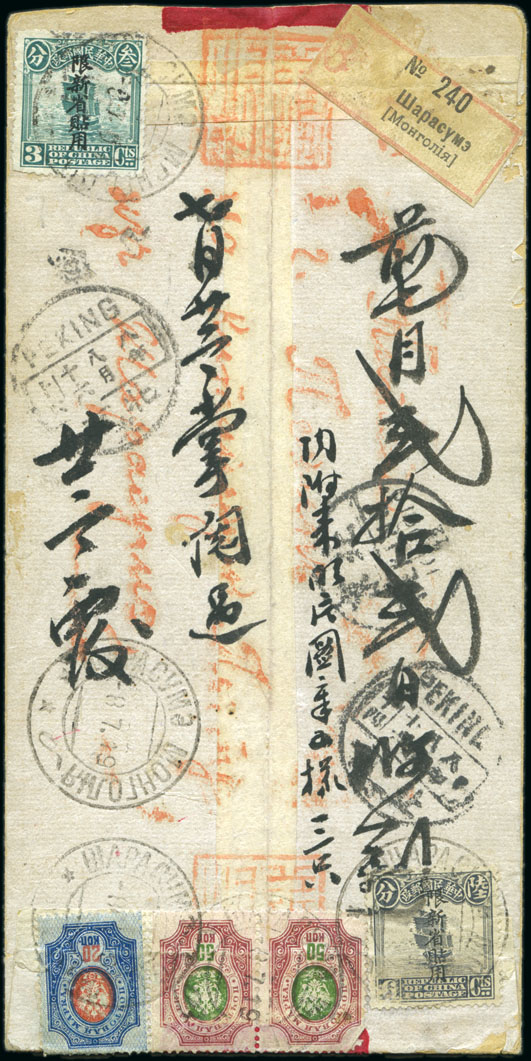
\includegraphics[width=.50\textwidth]{../russian-post-in-mongolia/10153.jpg}
\caption{ 
10153	SHARASUME: 1919 Native cover sent registered to Peking, with 20k
and pair of 50k in combination with Chinese 1c (on obverse), 3c and 6c, all
tied by the Sharasume 8.7.19 cds, with registration label adjacent 
(Hellrigl type 9 rated R), with Russian and Chinese Peking arrival ds, 
the double franking was imposed by the Chinese authorities in 
Sinkiang (to which Sharasume had been ceded) who no longer accepted
the validity of Russian stamps, a rare mixed country combination and a high franking.
Provenance: Ex Adgey-Edgar
\euro 6,000.00
} 
\end{figure}

\begin{figure}[htbp]
\centering
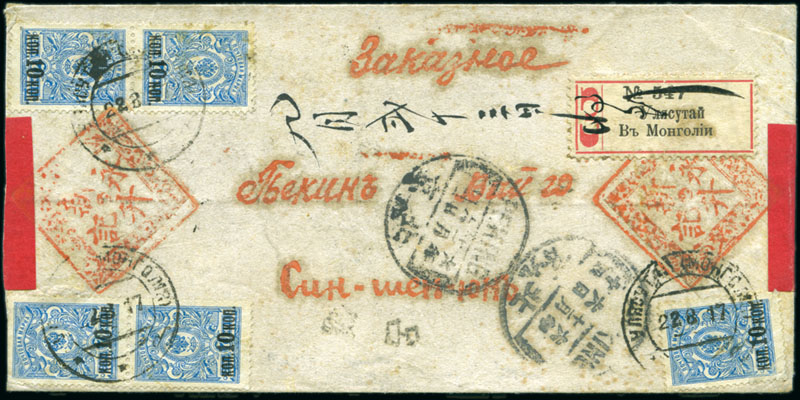
\includegraphics[width=.95\textwidth]{../russian-post-in-mongolia/10154.jpg}
\caption{ 
10154	ULYASUTAI: 1916 Native cover sent registered to Peking, franked with 
five 1916-17 10k on 7k blue paying double the 15k internal rate plus 20k 
registration fee, tied by Ulyasutai 22.8.17 type 2 cds, with registration 
label adjacent (Hellrigl type 2b rated RR), with Peking and Manchuli 
transits, fine and very rare, only six known covers from this Office.

Note: Taken by mounted courier to Khatkhyl, thence by Russian steamer 
across Lake Koso-Gol to Khanginsk, to the frontier post at Mondy and 
from there into the Russian rail network at Irkutsk for transmission 
by Trans-Siberian line to Chinese P.O. at Manchuli. Recorded in the 
British Journal of Russian Philately 37 (1965)
Provenance: Ex Holcombe
\euro 8,000.00
} 
\end{figure}

\begin{figure}[htbp]
\centering
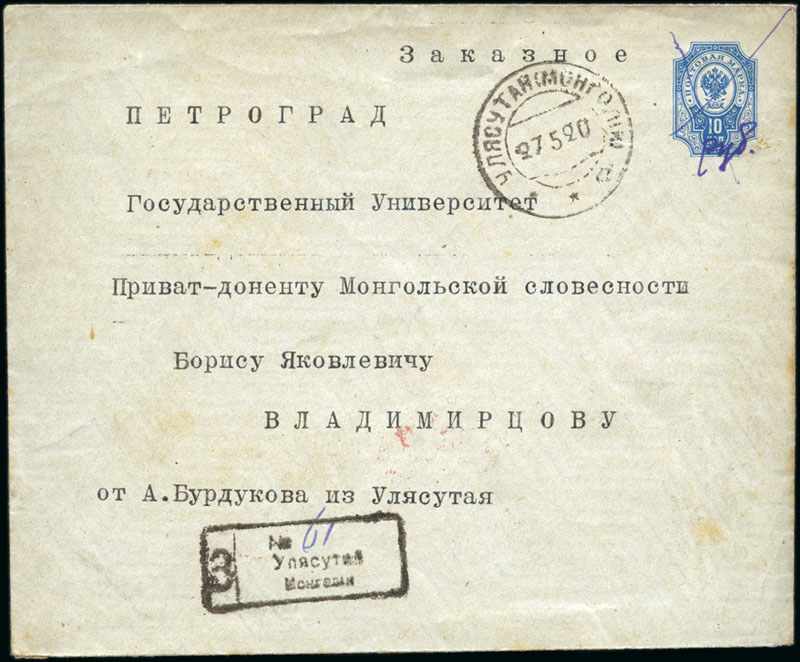
\includegraphics[width=.95\textwidth]{../russian-post-in-mongolia/10155.jpg}
\caption{ 
10155	ULYASUTAI: 1920 10k Postal stationery envelope surcharged in ms "rub" (roubles) to pay the correct registered rate in depreciated currency, sent to Petrograd, cancelled by pen with Ulyasutai 27.5.20 type 2A cds (Hellrigl rated RRR, believed to be unique) adjacent, plus registration hs (rated RRR, also believed to be unique), Pertrograd bs, very fine and unique, also believed to be the latest date recorded of the entire Russian period, cert. British Society of Russian Philately.

Note: Illustrated in "The Postal History of Mongolia" p.69 by Hellrigl and described as one of the rarest items of Mongolia's postal history
\euro35,000.00
} 
\end{figure}

\begin{figure}[htbp]
\centering
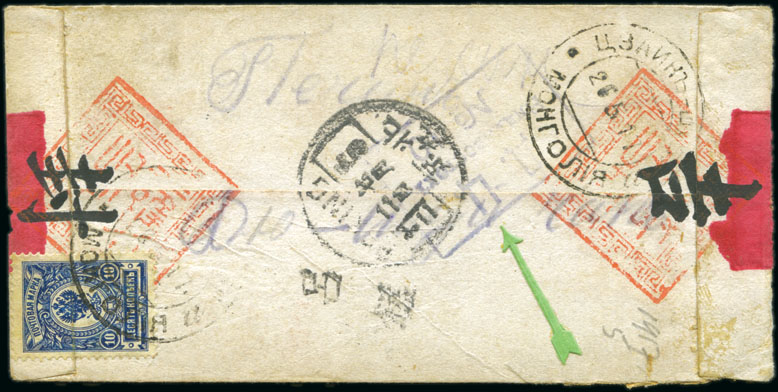
\includegraphics[width=.95\textwidth]{../russian-post-in-mongolia/10156.jpg}
\caption{ 
10156	TSAIN-SHABI: 1917 Native cover to Peking, franked with 10k blue paying
the single letter rate, tied by Tsain-Shabi 26.5.17 cds (the last recorded use
in black according to Hellrigl), with violet Vladivostok censor hs adjacent, 
fine and rare
\euro 1,800.00 
} 
\end{figure}

\begin{figure}[htbp]
\centering
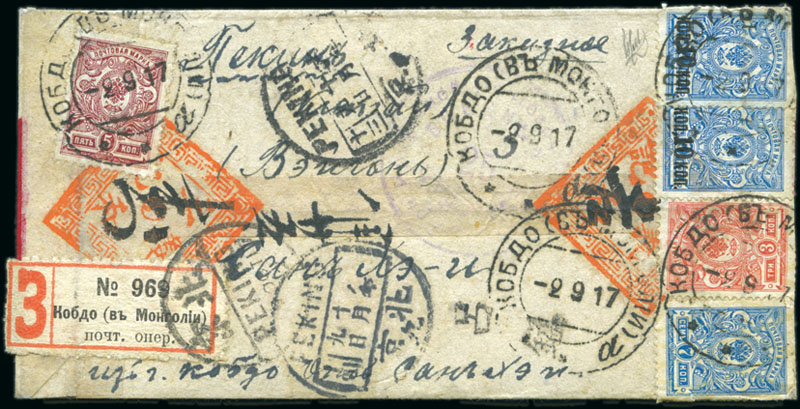
\includegraphics[width=.95\textwidth]{../russian-post-in-mongolia/10157.jpg}
\caption{ 
10157	KOBDO: 1917 Native cover sent registered to Peking, franked with 
Arms 3k, 5k and 7k plus two 1916 10k on 7k, paying the 15k single letter 
rate plus registration (despite the letter rate increasing to 20k the day 
before according to Hellrigl), tied by Kobdo 2.9.17 type 1A cds (Hellrigl rated RR), 
with reg'n label adjacent (type 1 rated RRR), Irkutsk censor hs, fine and very rare.

One of only four covers recorded from Kobdo and one of the great rarities
of Mongolian postal history.

Note: Illustrated in "The Postal History of Mongolia" pg.59 by Hellrigl

Expertise: Signed Holcombe

Provenance: Ex Tolman

\euro 70,000.00 
} 
\end{figure}

Lorem ipsum dolor sit amet, consectetur adipiscing elit. Sed nibh justo, dictum sed cursus ac, lobortis et lacus. Vestibulum vitae justo enim. Quisque laoreet elementum felis, ut sodales arcu viverra a. Sed molestie odio vulputate sem rutrum a sagittis est rutrum. Morbi dapibus hendrerit magna, sit amet commodo massa posuere sit amet. Duis pharetra quam scelerisque est lobortis fringilla. Maecenas venenatis feugiat lectus, vel facilisis odio pharetra quis. Etiam at nisl eros, sit amet suscipit lorem. Lorem ipsum dolor sit amet, consectetur adipiscing elit. Sed augue nunc, ornare eget congue sit amet, laoreet vel augue. Morbi vel justo quis ipsum adipiscing egestas vitae non est. Vivamus ac quam quam. Nullam pharetra
                                                    interdum mauris, rutrum pulvinar ligula condimentum id. Donec et blandit lorem. 

\begin{figure}[htbp]
\centering
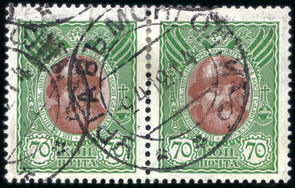
\includegraphics[width=.60\textwidth]{../russian-post-in-mongolia/10158.jpg}
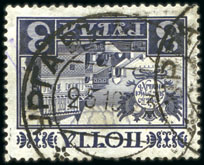
\includegraphics[width=.30\textwidth]{../russian-post-in-mongolia/10158-1.jpg}
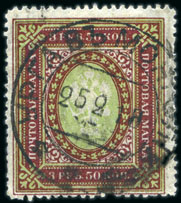
\includegraphics[width=.35\textwidth]{../russian-post-in-mongolia/10158-2.jpg}
\caption{ 
10158	Selection of stamps with different cancels incl. Urga type 7A (eight incl.
1912-18 1R pair, 3R50, Romanov 70k pair, 20k, 50k and 3R), Urga type 7B (1912-18 1R),
Ulyasutai type 2 (three 1912-18 1R) and Sharasume cds (Romanov 14k), odd minor fault,
a scarce group

(Image 1) (Image 2) (Image 3)	

Currently (SAN)...\euro 200.00 
} 
\end{figure}






                        